        
\documentclass{report}
\usepackage{hyperref}
\usepackage{amsmath} 
\usepackage{graphicx}
%%%%%%%%%%%%%%%%%%%%%%%%%%%%%%%%%%%%%%%%%%%%


\title{Independent Project EE3025}
\author{GOUTHAM.AGV , EE17BTECH11001}
\date{29 Dec 2020}


%%%%%%%%%%%%%%%%%%%%%%%%%%%%%%%%%%%%%%%%%%%%

\begin{document}

\maketitle
\chapter{Introduction to Eda Playground}
\section {Blink Program}

\hspace*{0.5cm} Implementation of Blink program on Eda Playground(online simulator) can be found \href{https://www.edaplayground.com/x/esSx}{here} and GitHub link \href{https://github.com/gouthamagv/FFT-FPGA-GVV/tree/main/blink}{here}\\.\par
A short video explanation of working with the simulator and code can be found  \href{https://youtu.be/i72Db3KiXbg}{here}.
\section{Seven Segment display counter}
\hspace*{0.5cm}Implementation of Seven segment display counter on Eda Playground can be found \href{https://www.edaplayground.com/x/7YHZ}{here} and GithuB link \href{https://github.com/gouthamagv/FFT-FPGA-GVV/tree/main/7_segment_display}{here}\\.\par
A short video explanation of working with the simulator and code can be found  \href{https://youtu.be/yMpw_An-A4w}{here}.
\begin{figure}[h]
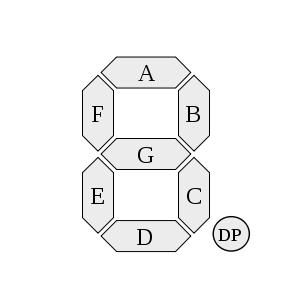
\includegraphics[scale=0.32]{B.png}
\centering
\end{figure}
\chapter{FFT Algorithm}
\section{Background}
Let x[n] be a series of complex signals, for 0$\leq$n$\leq$N-1 and X[k] the Discrete Fourier Transform of 0$\leq$k$\leq$N-1. The frequency domain signals X[k] can be obtained according to \emph{equation 2.2} or in its matrix form as can be seen in \emph{equation 2.3}, where 
\begin{equation}
    W_N^kn =exp(\frac{2ikn\pi}{N})
\end{equation}
\begin{align}
   X[k]=\sum_{n=0}^{N-1} X[n]W_N^kn
\end{align}
\begin{equation}
\begin{bmatrix} 
    X[0]  \\
    \vdots  \\
    X[k] 
    \end{bmatrix} =\begin{bmatrix} 
    W_N^{0*0} &  \dots    & W_N^{0 * N-1}   \\
    \vdots & \ddots  & \vdots \\
    W_N^{n-1 * 0} & \dots       & w_N^{N-1 * N-1} 
    \end{bmatrix} *\begin{bmatrix} 
    x[0]  \\
    \vdots  \\
    x[k] 
    \end{bmatrix}
\end{equation}
The computation of X[k]has complexity of $0$(n\textsuperscript{2}). However, the expression of the equation 2.2 may be split in two terms according to equation 2.4.
\begin{equation}
    X[k]=\sum_{n=0}^{N-1} X[2n]W_N^{2kn} + \sum_{n=0}^{N-1} X[2n+1]W_N^{2kn+1}
\end{equation}
Note that applying the properties  $W_N^{2kn}= W_{N/2}^{kn}$
and $W_N^{k+N/2}= -W_{N}^{kn}$ in the above equation, we get 
\begin{equation}
\begin{aligned}
  X[K]=Xe[k]+W_N^{k} Xo[k] \\
  X[K+N/2]=Xe[k]-W_N^{k} Xo[k] 
\end{aligned}
\end{equation}
where 
\begin{align*} 
Xe[k]=\sum_{n=0}^{\frac{N}{2}-1} X[n]W_\frac{N}{2}^{kn} \\
Xo[k]=\sum_{n=0}^{\frac{N}{2}-1} X[2n+1]W_\frac{N}{2}^{kn}
\end{align*}
According to equation 2.5, if N is a power of 2, the computation of X[k] has complexity of $0$(N*log\textsubscript{2}(N)).
\section{Recursive Algorithm}
A very simple algorithm to compute the FFT can be defined taking advantage of the recursive nature of the FFT, as can be seen in\\
\begin{figure}[h]
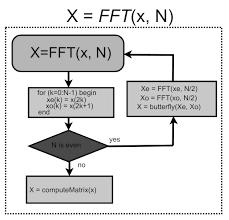
\includegraphics[scale=0.75]{download1.png}
\centering
\end{figure}
\par
if the size N of the FFT is even then call two FFT of order N/2, one to compute the Fourier Transform of the signals with even index (x[2n]) and other to compute the signals with odd index (x[2n+1]). \\The Fourier Transform will be scaled with the twiddle factor W\textsubscript{N}\textsuperscript{k}.
\begin{figure}[h]
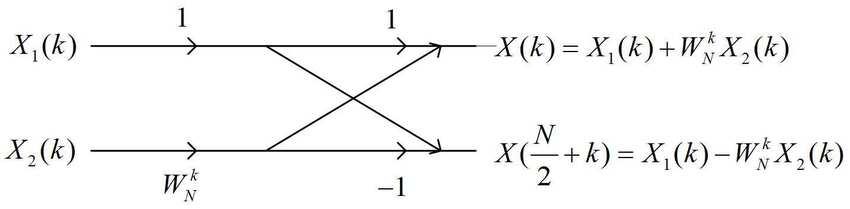
\includegraphics[scale=0.3]{butterfly-operation.png}
\centering
\end{figure}
if N is odd then the FFT will be slowly calculated using the Fourier matrix of equation 2.3(Matrix multiplication).\par
If the length N of the FFT is of the form N= m * 2\textsuperscript{p}, the the complexity of the algorithm of Figure 1 will be $O$(m\textsuperscript{2})×$O$(P * log\textsubscript{2}(p)).
Sudo code of the above algorithm considering genenral case m=1 is 
\begin{figure}[h]
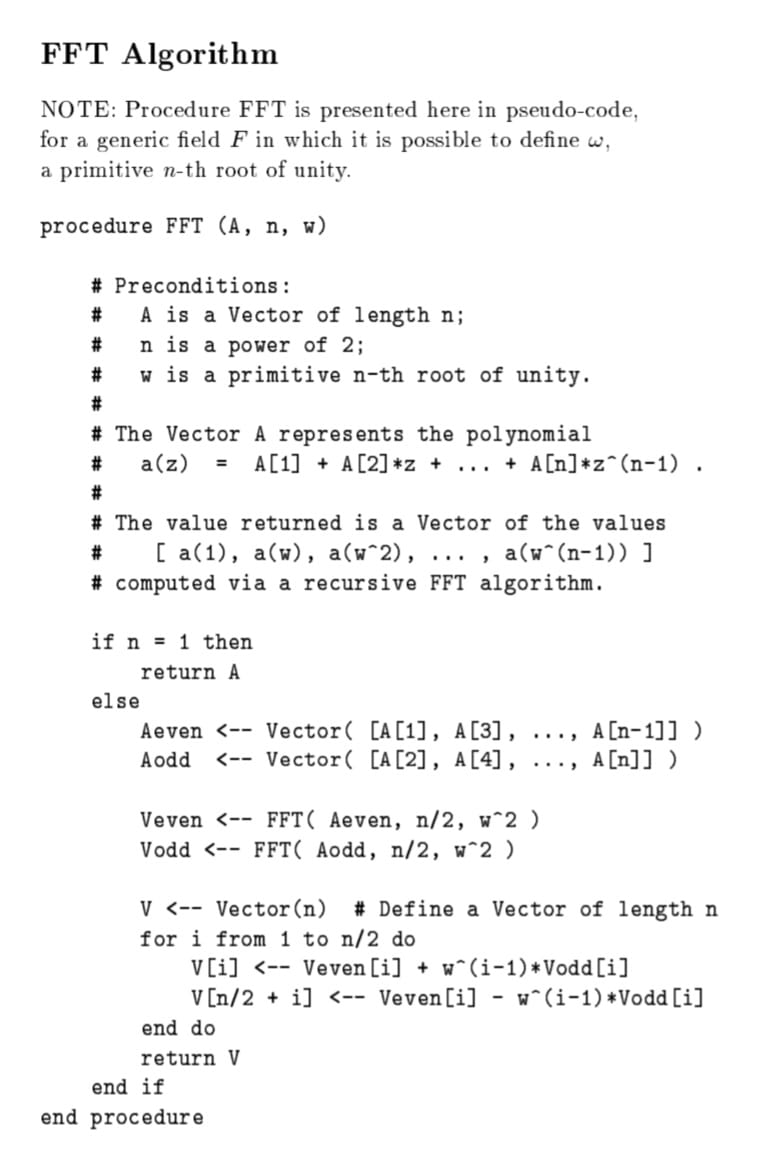
\includegraphics[scale=0.25]{A.jpeg}
\centering
\end{figure}
\section{Code and Links}
SystemVerilog code implemented in Eda Playground can be found \href{https://www.edaplayground.com/x/BaB5}{here} and corresponding GitHub link is \href{https://github.com/gouthamagv/FFT-FPGA-GVV/tree/main/FFT_in_verilog}{here}.\\
A short video explaining the recursive fft code using SystemVerilog can be found \href{https://youtu.be/lhDAXMt5oSE}{here}. \\
A faster algorithm iterative FFT is implemented in c code; Github link for c is \href{https://github.com/gouthamagv/FFT-FPGA-GVV/blob/main/FFT_iterative.c}{here}.\\
 \textbf{Github Link for all the codes in project is \href{https://github.com/gouthamagv/FFT-FPGA-GVV}{here}}.
\end{document}

    
